\chapter{Filtrage}

\paragraph*{Idée générale}
Le but de ce chapitre est de décrire les différentes méthodes de filtrage investiguées, dans le but d'améliorer la qualité des données.

\paragraph*{Problème}
Le dataset original est composé de 18 caméras regroupant environ 1 million d'images. Une bonne partie de ces images sont des faux positifs. Il est donc nécessaire de filtrer les images afin de ne garder que les images qui nous intéressent. Une première observation nous fait remarquer que les images uniquement constituées de feuilles n'ont jamais d'animaux. Ensuite, une deuxième lecture nous fait remarquer que les animaux se déplacent plus facilement par temps humide. Et finalement, nous constatons que les animaux sont nombreux à certains moments. À partir de ces observations, nous avons élaboré 3 méthodes pour filtrer les images et ainsi augmenter notre probabilité de trouver des animaux pour constituer de nouveaux labels ou constituer un dataset de validation.
Ces méthodes sont décrites dans les sections suivantes.

% -------------------------------

\section{Analyse des données labellisées}

Comme dit en introduction, notre professeur monsieur Satizabal Mejia Hector Fabio nous a fourni les bounding box pour certaines images. C'est sur le fichier `path\_and\_bounding\_box.csv`' - que nous avons préalablement créé à partir de ces données - que nous avons effectué l'analyse exploratoire des données. Nous nous basons ainsi 2020 images dont :

\begin{enumerate}
    \item[-] 224 observations de tritons ;
    \item[-] 201 observations de grenouilles-crapauds.
\end{enumerate}

\noindent Ces données s'étendent sur la période du 9 mars au 15 avril 2017. Il est premièrement important de noter que les données contenant des tritons et/ou des grenouilles-crapauds s'étendent du 9 mars au 1er avril, c'est-à-dire que l'on en a pas observé entre le 1er avril et le 15 avril. Nous avons donc observé la présence de tritons et/ou grenouilles-crapauds au travers de ces données via des variables temporelles - heure et jour - et via des variables météorologiques - telles que humidité, température ou précipitation. \newline

Aussi, il est important de noter ici que plusieurs images peuvent faire partie du passage du même animal; l'ensemble de données compte en effet 425 images mais beaucoup moins de séquence puisque une séquence est composée de plusieurs images. C'est pourquoi nous resterons très généraux pour cette première analyse des données. Voici donc ce que l'on a observé sur les données contenant des tritons et/ou des grenouilles-crapauds :

\subsection{Analyse temporelle}

\subsubsection{Date}

\begin{figure}[H]
    \centering
    \fbox{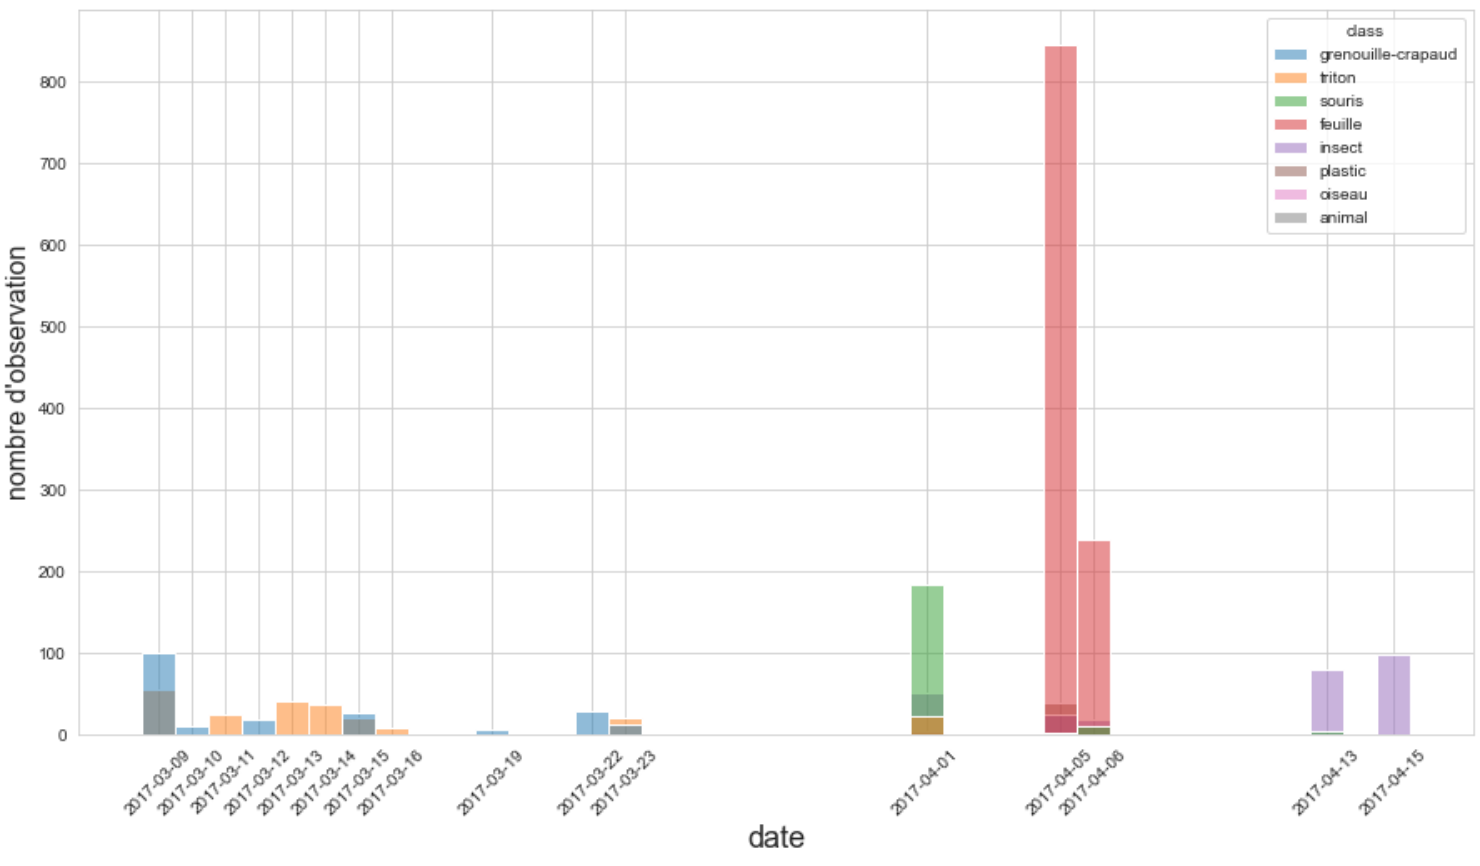
\includegraphics[width=300px]{images/filtre_observations_date.png}}
    \caption{Fréquentation des animaux en fonction de la date}
    \label{fig:Fréquentation des objets en fonction de la date}
\end{figure}

\begin{figure}[H]
    \centering
    \fbox{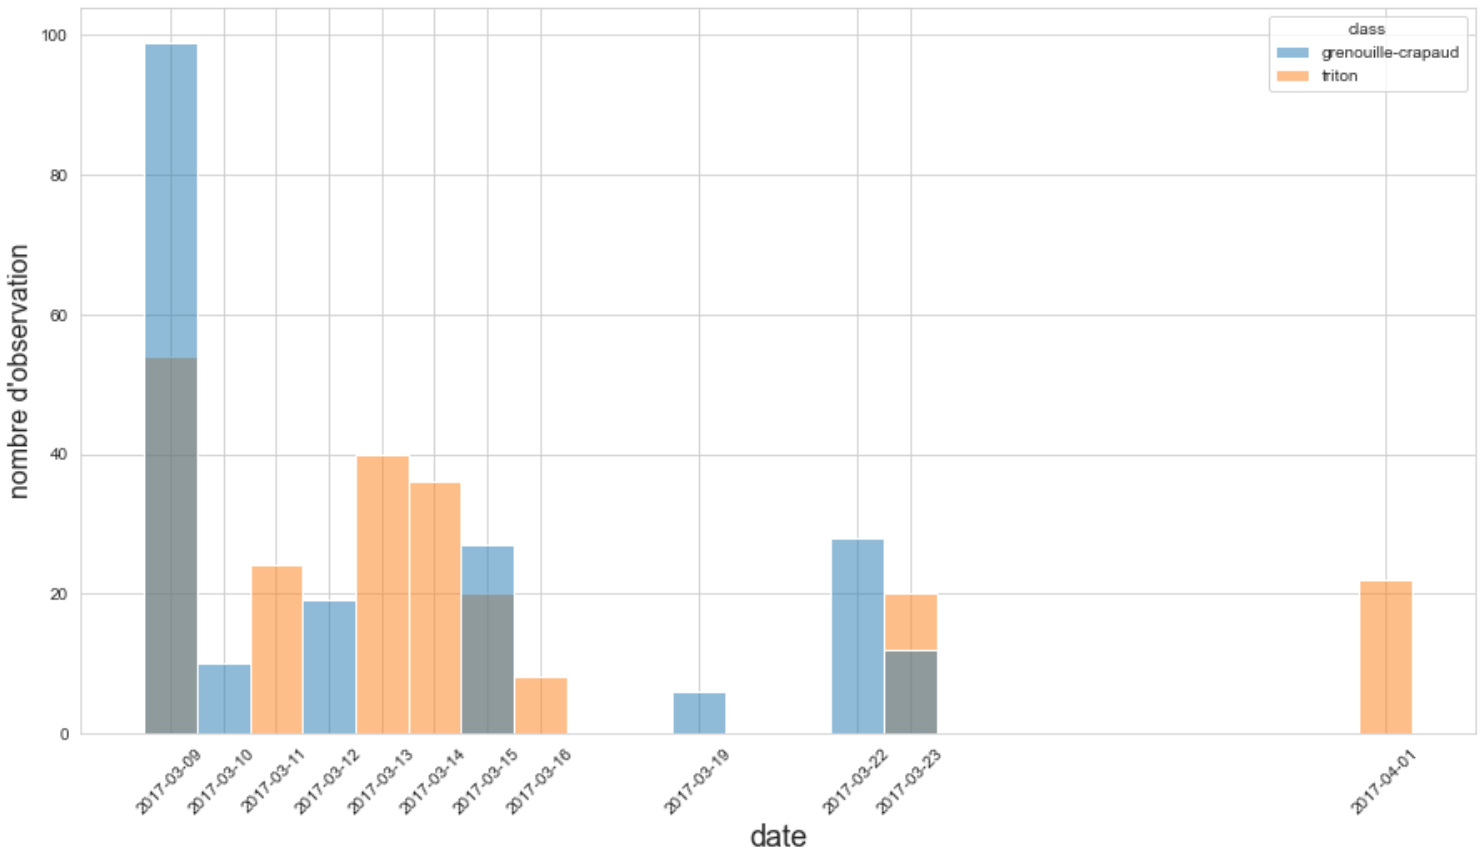
\includegraphics[width=300px]{images/filtre_crapGren_trit_date.png}}
    \caption{Fréquentation des batraciens observés en fonction de la date}
    \label{fig:Fréquentation des crapauducs en fonction de la date}
\end{figure}

\noindent On observe donc d'après la figure \ref{fig:Fréquentation des crapauducs en fonction de la date} que les batraciens d'intérêt utilisent particulièrement les crapauducs en mois de mars. Le reste des observations durant cette période, nous indique cependant que l'on observe peu de données en avril. \newline

Cependant, d'après cette ressource \footnote[1]{http://www.karch.ch/karch/home/amphibien/osservazione-di-anfibi.html} sur internet, les batraciens se reproduisent en fin février-début mars. On peut donc considérer que la déduction de fréquentation plus élevée des crapauducs par les batraciens en mars peut être considérée pour un premier filtrage pertinent des images.

\subsubsection{Heure}

\begin{figure}[H]
    \centering
    \fbox{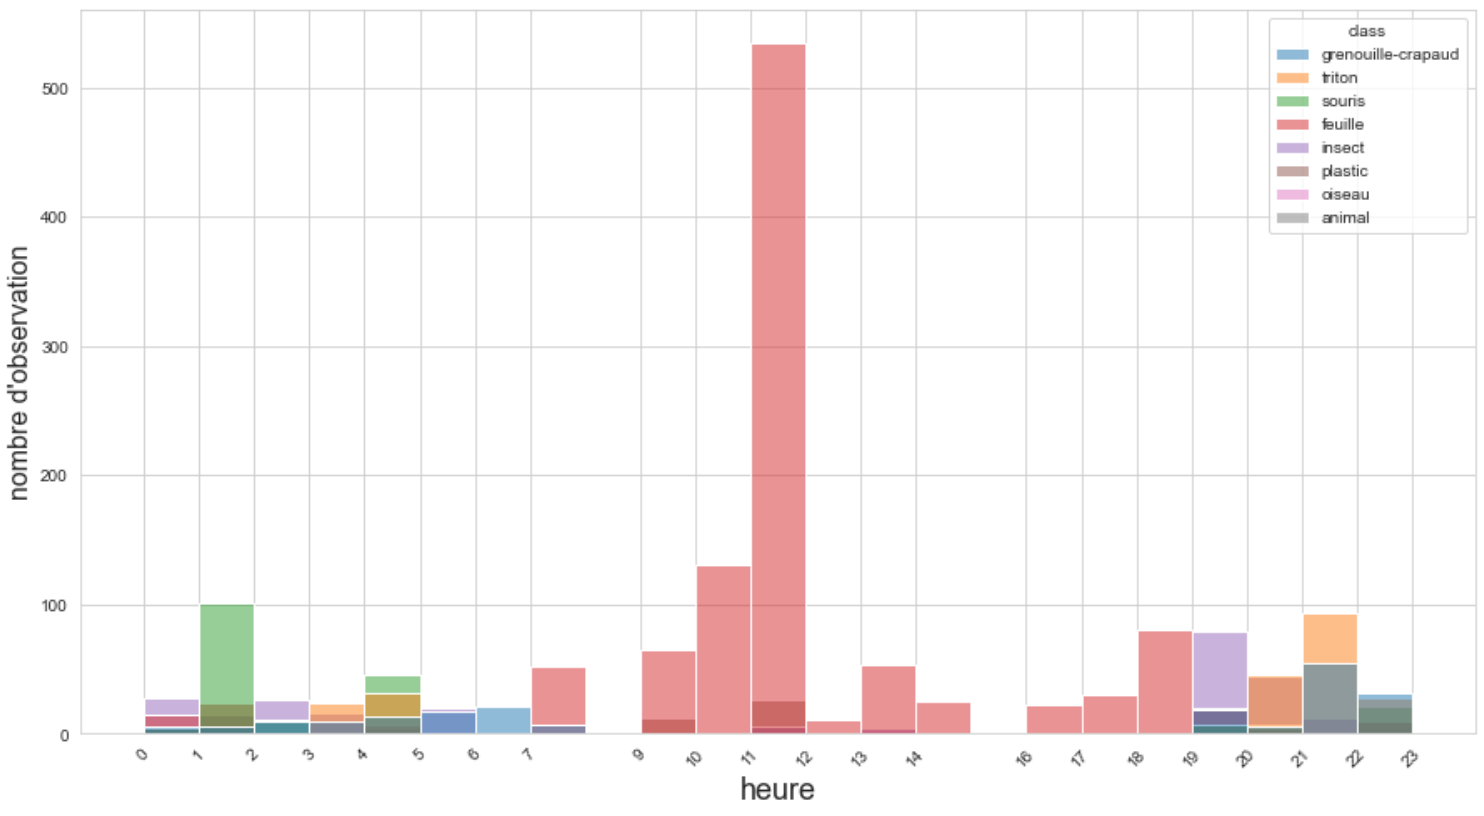
\includegraphics[width=300px]{images/filtre_observations_heure.png}}
    \caption{Fréquentation des animaux en fonction de l'heure}
    \label{fig:Fréquentation des objets en fonction de l'heure}
\end{figure}

On constate ici que le nombre de feuille étant plus grand que le reste d'objets observés, ceci nous empêche de pouvoir observer clairement la distribution d'observation d'objets. Visualisons donc les observations d'objets excepté les feuilles :

\begin{figure}[H]
    \centering
    \fbox{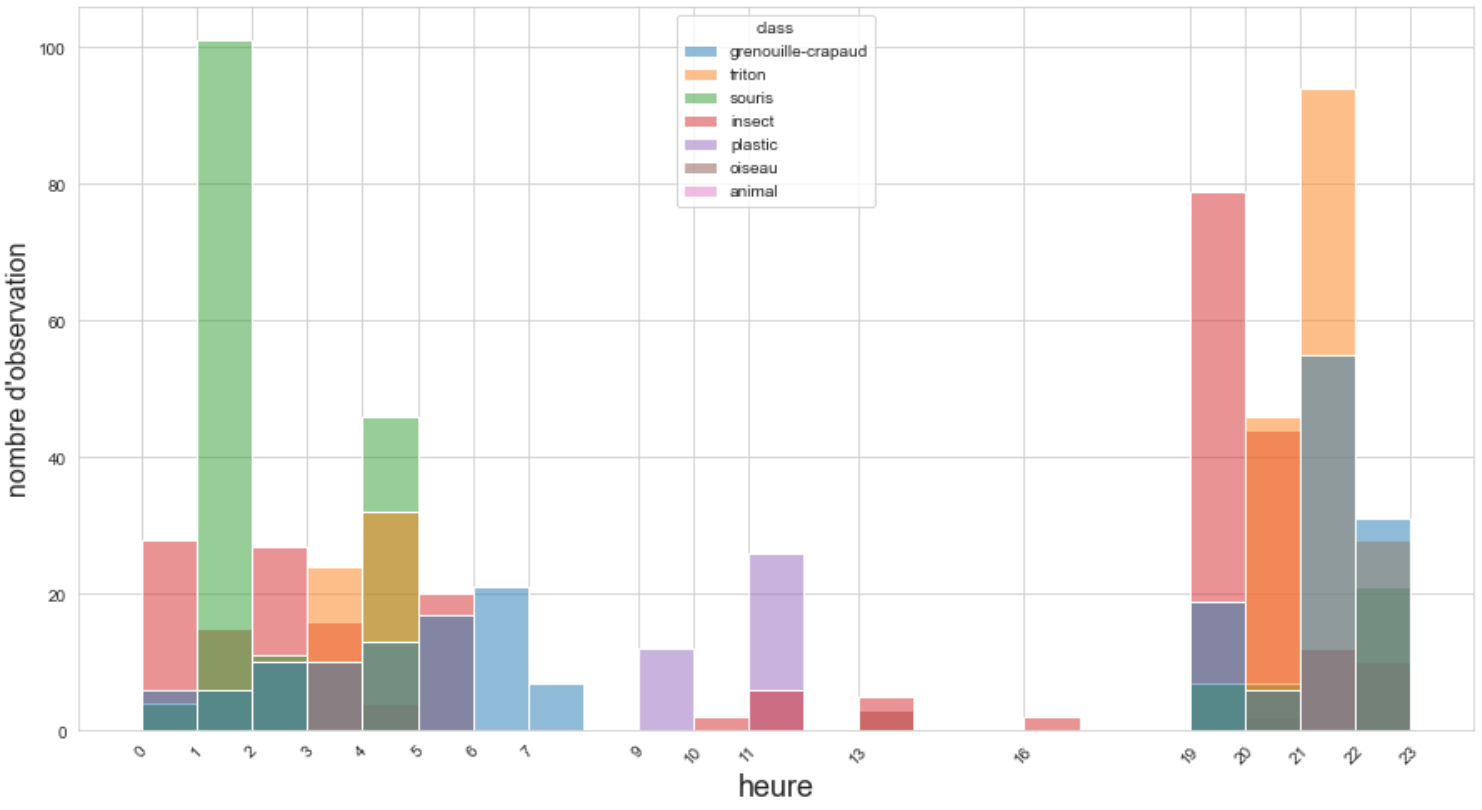
\includegraphics[width=300px]{images/filtre_observations_heure_sans_feuilles.png}}
    \caption{Fréquentation des batraciens observés en fonction de l'heure - sans les feuilles}
    \label{fig:Fréquentation des crapauducs en fonction de l'heure - sans les feuilles}
\end{figure}

\begin{figure}[H]
    \centering
    \fbox{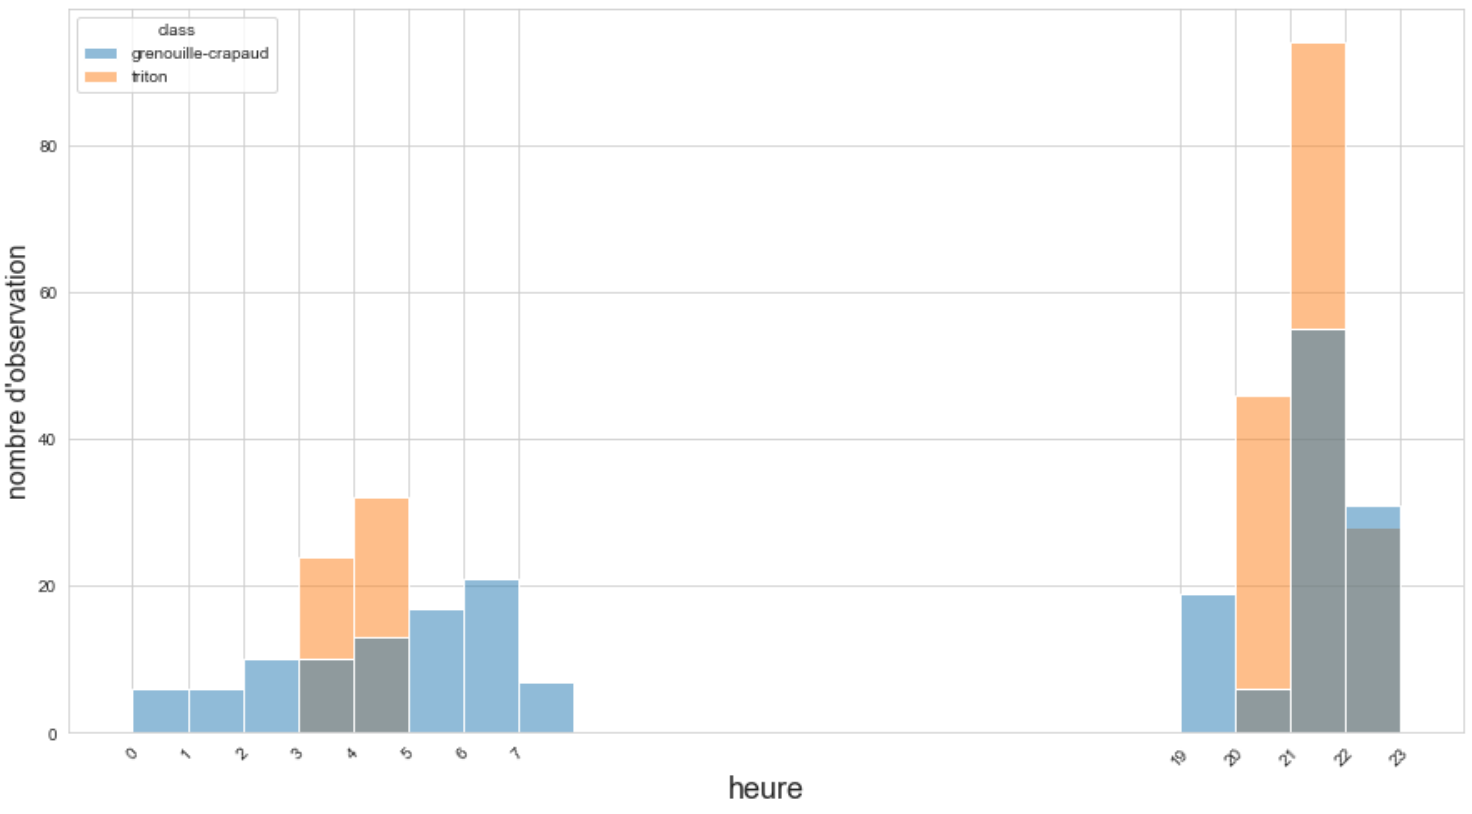
\includegraphics[width=300px]{images/filtre_crapGren_trit_heure.png}}
    \caption{Fréquentation des batraciens observés en fonction de l'heure}
    \label{fig:Fréquentation des crapauducs en fonction de l'heure}
\end{figure}

\noindent D'après la figure \ref{fig:Fréquentation des crapauducs en fonction de l'heure} ci-dessus, on observe que les batraciens d'intérêt utilisent particulièrement - même uniquement, pour cet ensemble de données - les crapauducs entre 19h et 7h du matin, c'est-à-dire de nuit. Le reste des observations (figure \ref{fig:Fréquentation des crapauducs en fonction de l'heure - sans les feuilles}) confirme premièrement la pertinence de cette observation, étant donné que nous avons une quantité élevée d'images prises tout au long de la journée parmi l'ensemble de données étudié ici.\newline

Les quelques recherches faites sur la période de déplacement des batraciens à l'étang indiquant également qu'elle est particulièrement durant le crépuscule, on confirme ainsi la pertinence que peut avoir ce deuxième filtrage des images.

% --

\subsection{Analyse météorologique}

Les données météorologiques additionnées des recherches en ligne ne sortent pas de particularité très prononcée quant à leur corrélation avec la fréquence d'observation de batraciens. Si l'on souhaite cependant citer les facteurs météorologiques qui pourraient être la plus déterministe, on citera l'humidité ; nous allons donc ici exposer nos observations la concernant. Notons que nous avons ici décidé de négliger les données labelisées "feuilles", comme elles forment du bruit et que nous avons fait un autre filtre s'en occupant si besoin.

\subsubsection{Humidité}

\begin{figure}[H]
    \centering
    \fbox{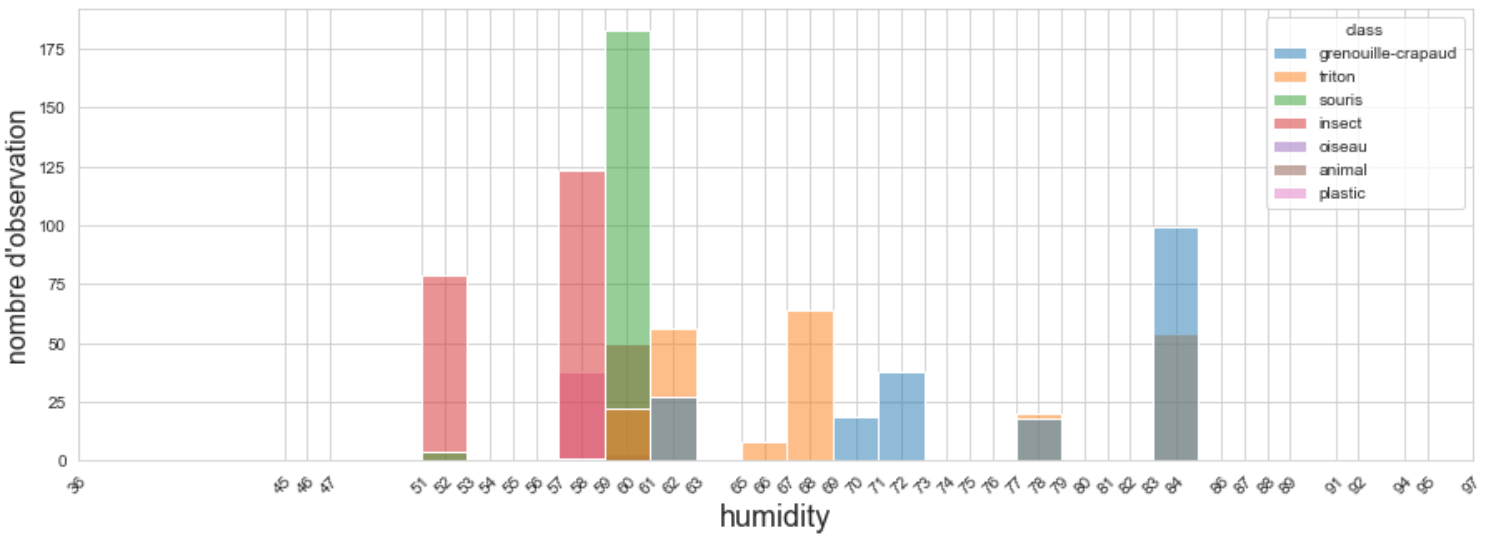
\includegraphics[width=300px]{images/filtre_meteo_observations_humidite.png}}
    \caption{Fréquentation des objets en fonction de l'humidité - sans les feuilles}
    \label{fig:Fréquentation des objets en fonction de l'humidité - sans les feuilles}
\end{figure}

\begin{figure}[H]
    \centering
    \fbox{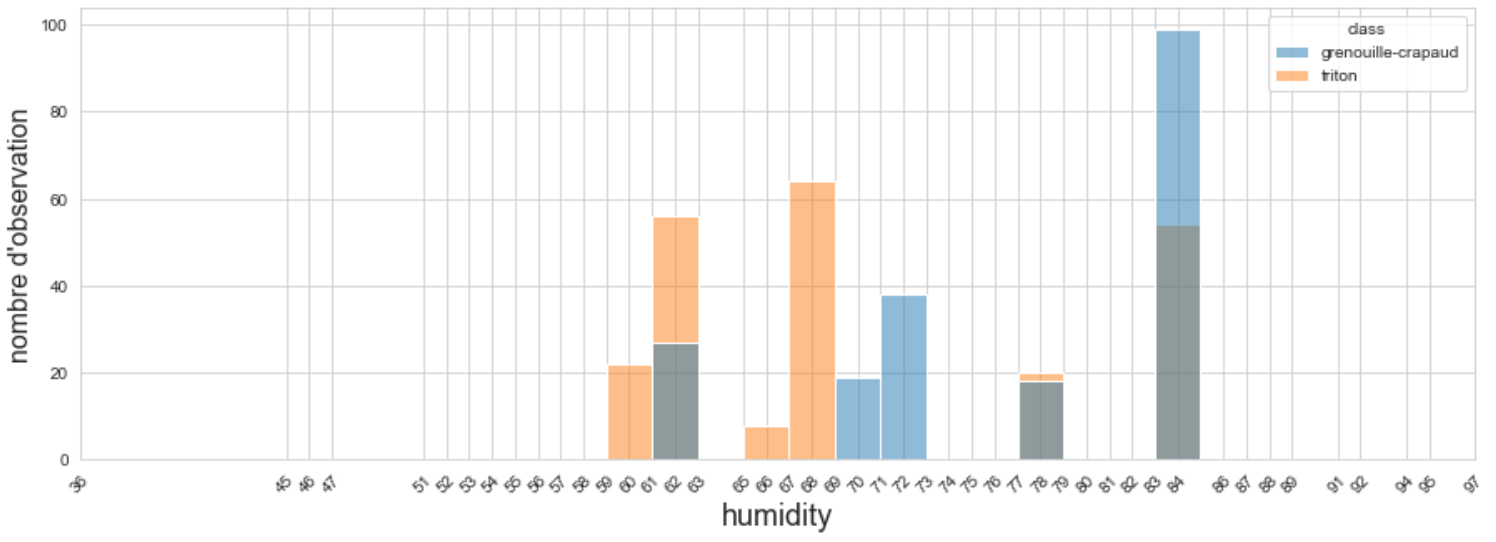
\includegraphics[width=300px]{images/filtre_meteo_crapGren_trit_humidite.png}}
    \caption{Fréquentation des batraciens en fonction de l'humidité - sans les feuilles}
    \label{fig:Fréquentation des batraciens en fonction de l'humidité - sans les feuilles}
\end{figure}

On voit ici qu'on peut imaginer prendre seulement les images prises lorsque l'humidité est au-dessus de 55.

% -------------------------------

\section{Détecteur de planches}\label{sex:Planche}

Nous avons développé un réseau de neurones convolutif à l'aide de la libraire PyTorch. Ce classificateur binaire, prédit ou non la présence de planche.

\paragraph*{Dataset d'entraînement}

Nous avons extrait 600 images d'une même caméra et labellisé 359 non planches et 241 planches. Ensuite, nous avons développé un dataloader permettant d'intégrer nos labels et de charger des batchs de données directement dans la libraire PyTorch. Celui ci, utilise un pipeline d'entrée qui applique plusieurs transformations à l'image avant de pouvoir l'utiliser comme un tenseur.

\begin{figure}[!htb]
    \centering
    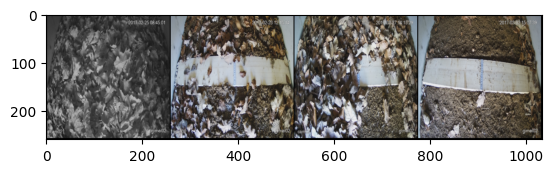
\includegraphics[width=200px]{images/filtre_exemple_data}
    \caption{Exemple de données d'entraînement}
    \label{fig:Entraînement du filtre}
\end{figure}

\paragraph*{Architecture du Détecteur}

Le détecteur est simplement constitué de 3 couches convolutives suivi de 2 couches entièrement connectées. Les channels d'entrée et de sortie des couches convolutives est de : 3 - 32, 32 - 64, 64 - 128. Le nombre de neurones des couches fully connected sont de 128 et 1 pour le neurone de sortie. La fonction de coût utilisé est la BCELoss et l'optimiseur est Adam. Le réseau est entraîné pendant 10 epochs avec un learning rate de 0.001 et un momentum de 0.9 sur 3 epochs.

\begin{figure}[!htb]
    \centering
    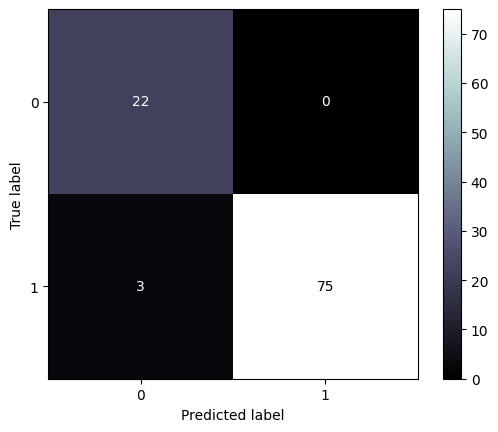
\includegraphics[width=200px]{images/filtre_cmatrix}
    \caption{Matrice de confusion du détecteur de planche}
    \label{fig:Matrice de confusion du filtre}
\end{figure}

\paragraph*{Résultats}

Le détecteur de planche a une précision de 1 et un recall de 0.98 sur la détection de planche. En revanche, la précision sur la détection de non planche est de 0.88 et un recall de 1. Ce qui veut dire que notre filtre est un peu trop efficace et a tendance à se tromper pour détecter les images sans planche. Comme les résultats sont satisfaisant pour dégrossir le travail, nous n'avons pas passé de temps supplémentaire à optimiser le réseau afin qu'il sépare mieux les images dotés d'une planche ou non. Comme, nous traitons une grande quantité de données, l'erreur est acceptable. Lancé sur la quasi intégralité du dataset, le filtre a tourné pendant plus de 10h sur un ordinateur de bureau doté d'un processeur Ryzen9500X. Au final, le filtre a détecté 48910 images de non planches sur les 754543 images analysées.